\chapter{食物的旅程}\label{ch:g4:journey-of-food}

一口面包：嚼碎、咽下——就不见了。去了哪里？到
今晚，这口面包的一部分会帮助你的腿奔跑、骨头生长，
这意味着它必须设法从吞下它的管子里\emph{出}来，
再\emph{进入}身体的其余部分。
跟着这一口食物走一走：它的旅程
是身体里最精彩的故事之一。

\section{消化道}

\begin{definition}[消化道]\label{def:g4:journey-of-food:tract}
食物沿着一根长管前行，
这根长管就是\emph{消化道}\index{消化道}，
它贯穿整个身体：
\begin{enumerate}
  \item \emph{口腔}\index{口腔}，牙齿在此磨碎食物
        （见\cref{ch:g2:teeth-and-eating-well}）；
        \emph{唾液}\index{唾液}使食物湿润；
  \item \emph{食道}\index{食道}，
        是从咽喉通向胃的一条滑道；
  \item \emph{胃}\index{胃}，一个\omterm{def:g3:bones-and-muscles:muscle}{肌肉}质的囊袋，
        食物在这里被搅拌，并与\omterm{def:g4:journey-of-food:digestion}{消化液}混合
        持续数小时；
  \item \emph{小肠}\index{小肠}，一根折叠的长管，
        长达数米，\omterm{def:g4:journey-of-food:digestion}{消化}在这里完成，
        食物中的有益成分进入身体；
  \item \emph{大肠}\index{大肠}，
        在这里从残留物中回收水分，
        然后残渣排出体外。
\end{enumerate}
\end{definition}

\begin{omfigure}
\begin{tikzpicture}
  \node[anchor=south west, inner sep=0] (img) at (0,0)
    {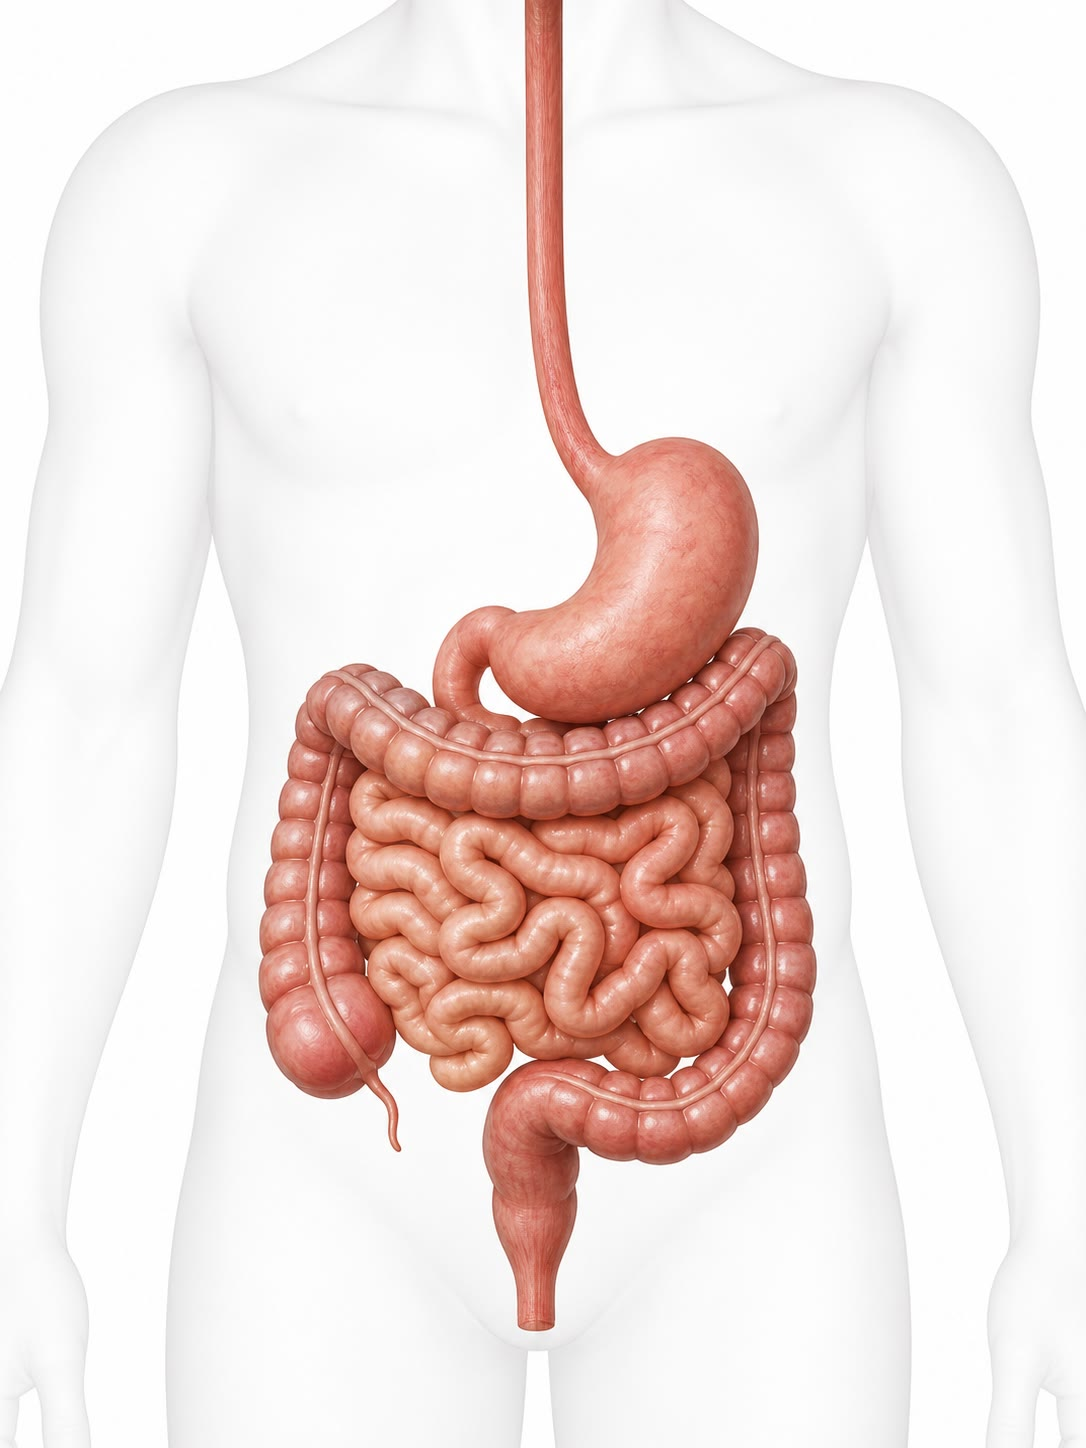
\includegraphics[width=0.5\linewidth]{images/book1/ai/fig-digestive.jpg}};
  \begin{scope}[x={(img.south east)}, y={(img.north west)},
      every node/.style={font=\small}]
    \draw[omDef, thick] (0.52,0.85) -- (0.72,0.88) node[right] {食道};
    \draw[omDef, thick] (0.66,0.62) -- (0.82,0.66) node[right] {胃};
    \draw[omDef, thick] (0.44,0.35) -- (0.16,0.28)
      node[left, align=center] {小肠 \\ （数米长，折叠）};
    \draw[omDef, thick] (0.74,0.42) -- (1.04,0.40)
      node[right, align=left] {大肠};
    \draw[omDef, thick] (0.50,0.09) -- (0.66,0.05)
      node[right] {残渣排出};
  \end{scope}
\end{tikzpicture}

{\small \omterm{def:g4:journey-of-food:tract}{消化道}：从口腔到出口的一根长管。\omterm{def:g4:journey-of-food:tract}{食道}
将食物送至胃；\omterm{def:g4:journey-of-food:tract}{小肠}折叠的数米长管子
位于中部，由\omterm{def:g4:journey-of-food:tract}{大肠}环绕。}
\end{omfigure}

\begin{example}[计算旅程的时间]\label{ex:g4:journey-of-food:timing}
这一口面包在口腔中停留几秒，
沿\omterm{def:g4:journey-of-food:tract}{食道}下滑约几秒，在胃里搅拌数小时，
再在\omterm{def:g4:journey-of-food:tract}{小肠}中经历好几个小时，
最后在\omterm{def:g4:journey-of-food:tract}{大肠}中完成，最长可达一天或更久。
整个旅程通常需要一到两天。
\end{example}

\section{消化：从食物到营养物质}

\begin{definition}[消化与营养物质]\label{def:g4:journey-of-food:digestion}
\emph{消化}\index{消化}是指食物沿\omterm{def:g4:journey-of-food:tract}{消化道}转化，
使其变成足够小、足够简单、能进入身体的成分，
即\emph{营养物质}\index{营养物质}。
牙齿咀嚼和胃的搅拌先将食物切碎；
\emph{消化液}\index{消化液}
——其中包括\omterm{def:g4:journey-of-food:tract}{唾液}——将其进一步分解，
逐步拆解，直到原来的面包变成
营养物质的液体混合物。
\end{definition}

\begin{example}[面包变甜]\label{ex:g4:journey-of-food:sweet}
把一小块普通面包嚼很久——慢慢数到六十——
就会尝到淡淡的甜味。没有加入任何东西：
\omterm{def:g4:journey-of-food:tract}{唾液}已经在把面包分解成更简单、更甜的小块。
你尝到的，正是\omterm{def:g4:journey-of-food:digestion}{消化}的开始。
\end{example}

\begin{proposition}[穿过进入身体]\label{prop:g4:journey-of-food:absorb}
\omterm{def:g4:journey-of-food:tract}{消化道}的内部在某种意义上仍在身体之外——
就像甜甜圈中间的孔。
\omterm{def:g4:journey-of-food:digestion}{营养物质}的穿越发生在\emph{\omterm{def:g4:journey-of-food:tract}{小肠}}中：透过\omterm{def:g4:journey-of-food:tract}{小肠}薄而深深折叠的管壁，
\omterm{def:g4:journey-of-food:digestion}{营养物质}进入\emph{血液}\index{血液}，
\omterm{prop:g4:journey-of-food:absorb}{血液}将其输送到身体的各个部分
（这一配送服务在\cref{ch:g4:heart-and-blood}中有所探讨）。
无法穿过的物质——纤维、外皮——
继续向前，在\omterm{def:g4:journey-of-food:tract}{大肠}中失去水分，
最后以粪便的形式排出体外。
\end{proposition}
\admitted

\begin{remark}[为何要折叠，为何有数米长]\label{rem:g4:journey-of-food:surface}
穿越管壁需要足够的表面积，\omterm{def:g4:journey-of-food:tract}{小肠}正是为此而构造：
长达数米，管壁一层层地折叠。
若把它摊平，这个吸收面积足以铺满一间小房间，
却紧紧装在腹中。身体里的大工程，
都靠把大面积折叠得很小来完成。
\end{remark}

\section{帮助消化顺利进行}

\begin{method}[有助消化的习惯]\label{met:g4:journey-of-food:habits}
\begin{enumerate}
  \item 认真咀嚼：胃里没有牙齿，口腔没有嚼碎的，
        胃就得费力去对付；
  \item 进餐要平静，定时进餐；
  \item 用餐时喝水；
  \item 多吃富含纤维的食物——蔬菜、水果、全麦面包：
        纤维能帮助残渣继续向前移动；
  \item 剧烈的游戏或游泳要等饭后\omterm{def:g4:journey-of-food:digestion}{消化}稳定之后再进行：
        用力工作的胃与用力运动的腿会彼此争夺
        身体的资源。
\end{enumerate}
\end{method}

\begin{example}[胃痛侦探]\label{ex:g4:journey-of-food:ache}
狼吞虎咽地吃完午饭，接着猛跑：典型的
下午胃痛。午饭没有嚼碎就咽下（违反第 1 条），
\omterm{def:g4:journey-of-food:digestion}{消化}中的胃又被催着去赛跑（违反第 5 条）。
解决办法不是吃药，而是讲礼貌——对待
自己的\omterm{def:g4:journey-of-food:tract}{消化道}要温和。
\end{example}

\section{练习}

\begin{exercise}[$\star$]\label{exo:g4:journey-of-food:1}
按顺序说出\omterm{def:g4:journey-of-food:tract}{消化道}的各个部分，从口腔到
出口。
\end{exercise}

\begin{exercise}[$\star$]\label{exo:g4:journey-of-food:2}
食物在胃里发生了什么变化，
大约在胃里停留多久？
\end{exercise}

\begin{exercise}[$\star$]\label{exo:g4:journey-of-food:3}
什么是\omterm{def:g4:journey-of-food:digestion}{消化}？什么是\omterm{def:g4:journey-of-food:digestion}{营养物质}？
\end{exercise}

\begin{exercise}[$\star$]\label{exo:g4:journey-of-food:4}
\omterm{def:g4:journey-of-food:digestion}{营养物质}在哪个部位进入\omterm{prop:g4:journey-of-food:absorb}{血液}？哪些物质
无法进入\omterm{prop:g4:journey-of-food:absorb}{血液}，又会怎样？
\end{exercise}

\begin{exercise}[$\star$]\label{exo:g4:journey-of-food:5}
为什么充分咀嚼的面包会带一点甜味？
\end{exercise}

\begin{exercise}[$\star$]\label{exo:g4:journey-of-food:6}
为什么\omterm{def:g4:journey-of-food:tract}{小肠}那么长，内部皱褶又那么多？
\end{exercise}

\begin{exercise}[$\star$]\label{exo:g4:journey-of-food:7}
列出三个有利于\omterm{def:g4:journey-of-food:digestion}{消化}的习惯，并说明每个习惯的原因。
\end{exercise}

\begin{exercise}[$\star$]\label{exo:g4:journey-of-food:8}
动手试一试（在餐桌上）：给下一顿饭计时。食物在口腔里停留了多久——
与它之后的\omterm{def:g4:journey-of-food:digestion}{消化}之旅相比，又如何？
它接下来要花上好几天的旅程，又该怎样看待？
\end{exercise}

\begin{exercise}[$\star\star$]\label{exo:g4:journey-of-food:9}
请诊断\cref{ex:g4:journey-of-food:ache}中的胃痛：
哪两个习惯被违反了，
明天你打算改变什么？
\end{exercise}

\begin{exercise}[$\star\star$]\label{exo:g4:journey-of-food:10}
“食物一吞下就进入了身体。”
请利用\cref{prop:g4:journey-of-food:absorb}加以纠正：
食物究竟在哪里进入身体？
在此之前，食物必须先经历什么？
\end{exercise}

\begin{exercise}[$\star\star\star$]\label{exo:g4:journey-of-food:11}
牛吃的草比你的面包坚韧得多，
而牛有四个胃室，会反刍，
并在肠道中寄居着帮助分解草料的有益\omterm{def:g1:living-or-not:living}{生物}。
利用\cref{def:g4:journey-of-food:digestion}和
\cref{prop:g2:what-animals-eat:match}，解释为什么以草为食的\omterm{def:g1:animals-around-us:animal}{动物}
需要这套更为复杂的\omterm{def:g4:journey-of-food:digestion}{消化}器官。
\end{exercise}
